%%%%%%%%%%%%
%
% $Autor: Wings $
% $Datum: 2019-03-05 08:03:15Z $
% $Pfad:  Wings-hub\210520PortentaH7\PortentaH7\$
% $Name: PortentaH7$
% $Version: 4250 $
%
%%%%%%%%%%%%


\section{Edge Impulse}

Edge Impulse is a platform which makes the process of machine learning easier by choosing reasonable defaults  for the parameters to be set when creating a model. It was founded in 2019 by Zach Shelby and Jan Jongboom. It provides a user friendly interface and we can train, test and deploy the model.Edge Impulse uses the TensorFlow ecosystem for training , optimizing and deploying deep learning models in to the embedded devices for example Arduino Portenta H7 \cite{EdgeImpulsedocs:2021}. The TensorFlow ecosystem provides a set of standards and integration points that can be used to make our own improvements in the model.

\begin{figure}[H]
	\centering
	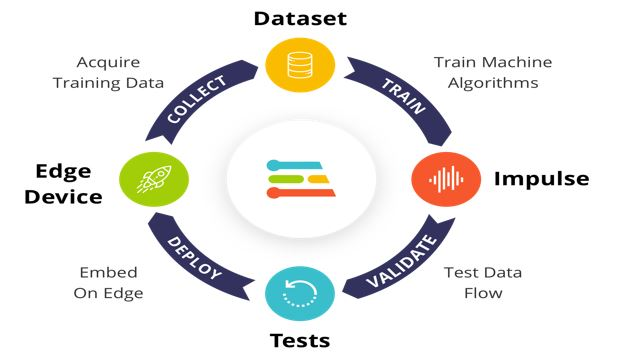
\includegraphics[width=\textwidth]{Arduino/edgeimpulse}
	\caption{Edge Impulse process \cite{EdgeImpulse:2021}}
	\label{figure 9.2.1}
\end{figure}


The process involves collecting  the data from the devices and creating a training data set in the Edge Impulse cloud. Then it will undergo the training process for the model and after the training process is completed, the model is tested using the testing data provided or the model can also be validated using live classification by loading the testing sample directly from a device. Then finally after the model is tested, it is deployed back in the device. 
In the background, Edge Impulse generates a python implementation of the model using TensorFlow ‘s Keras APIs. By switching into the expert mode we can edit the code and make changes in the parameters. The TensorFlow libraries and APIs are used by Edge Impulse and hence it makes it easy to extend the built-in training code with our own logic. The training process is done in the cloud and the trained model are automatically optimized for deployment to the microcontrollers.

\textbf{Data Acquisition format :}
In order to send data from any sensor to the Edge Impulse platform we need to send the data in data acquisition format. If the data we have is in CSV or WAV then we can directly upload in the Edge Impulse platform. For images,the input image formats accepted by the Edge impulse platform are JPG and PNG. Images can be in RGB or Grayscale. There is also an option available if we need to convert the input image into grayscale. 

\textbf{Image Processing Block : } In this processing block, preprocessing and normalization of image data is done. In addition, color depth can also be reduced. After the input image is loaded, this processing block is responsible for extracting features from the image.

\textbf{Learning Block : } In this learning block we have options to choose between classification and object detection.  The object detection model is a pre-trained model and we can use this pre-trained model and do fine tuning to obtain desired results. This pre-trained model is based on MobileNetV2-SSD FPN-lite architecture which is designed for mobile and embedded vision application. This model is trained on images of 320X320 resolution.


\textbf{Advantages }
\begin{itemize}
	\item 	Connect multiple devices to the platform. Even a mobile phone can also be used as a device.
	\item	Multiple options to upload our input data from different devices.
	\item	Drag and drop UI makes it user friendly for training, testing and deploying the model with little to no coding.
	
	\textbf{Disadvantages}
	\item	Difficult for fine grain customization of the model.
	\item	Data security issues.
	
	
\end{itemize}





